\documentclass[12pt, twoside]{report}

%Packages and Dependencies
\usepackage[utf8]{inputenc}
\usepackage{style}

\begin{document}

%%%%%%%%%%% Half Title
\thispagestyle{empty}
\vspace*{\fill}
\begin{center}
\textsc{\Large MULTI-PLATFORM GENOMIC DATA FUSION WITH INTEGRATIVE DEEP LEARNING}
\end{center}
\vspace*{\fill}
%%%%%%%%%%%%%%%%%%%%%

\setcounter{page}{0}
\clearpage

%%%%%%%%%%% Title page 
\thispagestyle{empty}
\begin{center}
    \vfill
    \textsc{\Large MULTI-PLATFORM GENOMIC DATA FUSION WITH INTEGRATIVE DEEP LEARNING}\\
    \vfill
    By Olatunji Oni, B.Sc. \\
    \vfill
    {\large \textit{A Thesis Submitted to the School of Graduate Studies in the Partial Fulfillment of the Requirements for the Degree Master of Science}}\\

    \vfill
    {\large McMaster University\, \copyright\, Copyright by Olatunji Oni\, \today}\\[4cm]
\end{center}
%%%%%%%%%%%%%%%%%%%%%%%

\newpage
\pagenumbering{roman}
\setcounter{page}{2}

\begin{singlespace}
    \noindent
    McMaster University \\ 
    Master of Science\, (\the\year) \\
    Hamilton, Ontario (School of Computational Science and Engineering) \\[1.5cm]
    TITLE: Multi-Platform Genomic Data Fusion with Integrative Deep Learning \\
    AUTHOR: Olatunji Oni\,  %list previous degrees
    (McMaster University)  \\
    SUPERVISOR: Dr. Sanzheng Qiao\, \\ 
    NUMBER OF PAGES: \pageref{lastoffront}, \pageref{LastPage}
\end{singlespace}

\clearpage
%%%%%%%%%%%%%%%%% ABSTRACT
\section*{\Huge Abstract} 
\addcontentsline{toc}{section}{Abstract}
 %Abstract goes here
\clearpage

%%%%%%%%%%%%% ACKNOWLEDGEMENTS
\section*{\Huge Acknowledgments} 
\addcontentsline{toc}{section}{Acknowledgments}
 %Acknowledgements
\clearpage

% \begin{singlespace}
% \end{singlespace}

\frontmatter{}
    \tableofcontents
    \listoftables
    \listoffigures
    \begin{table}[ht]
\caption{Summary of Mathematical Notations} % title of Table
\centering % used for centering table
\begin{tabular}{l l} % centered columns (4 columns)
\hline %inserts double horizontal lines
Symbol & Description \\ %[0.5ex] % inserts table
%heading
\hline % inserts single horizontal line
$X$ & A matrix. \\ % inserting body of the table
$\hat{y}$ & The model approximation from a neural network.  \\
$\theta$ & The variable weights in a neural network.  \\
$b$ & The bias terms in a neural network. \\  % [1ex] adds vertical space
$\Theta$ & The set of all parameters in a neural network.  \\
$J(\cdot)$ & A neural network cost function. \\
$\psi(\cdot)$ & An activation function. \\
$\alpha$ & An optimization learning rate. \\
$\tilde{x}$ & The noised version of input data $x$.  \\
$x'$ & The reconstruction of input data $x$ from an autoencoder.  \\
$g_{\theta}(\cdot)$ & The encoding function of an autoencoder.  \\
$f_{\theta^{T}}(\cdot)$ & The decoding function of an autoencoder.  \\ [1ex]
\hline %inserts single line
\end{tabular}
\label{table:notation}
\end{table}

    
    \pagenumbering{arabic}
    \pagestyle{fancy}
    \fancyhead{}
    \fancyfoot{}
    \fancyhead[RE,LO]{McMaster University --- Comput. Sci. \& Engineering}
    \fancyhead[LE,RO]{MSc Thesis --- Olatunji Oni}
    \fancyfoot[CE,CO]{\thepage}
    

\mainmatter{}
    \chapter{Background}\label{chap:background}

The background material in this chapter provides an overview of the theoretical concepts and fundamental technologies in which our deep learning approach is built. A few main concepts must be understood to appreciate the role of deep learning in data integration and predictive models. The first, and most fundamental to the discussion is an introduction to Artificial Neural Networks (ANNs), and their extension into the field of deep learning and information fusion. 

\section{Artificial Neural Networks}\label{sec:ann}
\subsubsection{Introduction}

Early attempts in designing computational systems to exhibit intelligent behaviour were conducted through formal rule-based programs referred to as Expert Systems~\cite{weiss1991computer}. In these systems, inference engines were used to apply a knowledge base of curated rules to deduce new rules and make predictions on future behaviour. It soon became evident that the sheer number of hard-coded rules required to simulate predictive behaviour was several orders of magnitude higher then capable to store or write for even moderately complicated tasks. This resulted in a shift from rigid and deductive systems towards inductive systems that learn to extract information from observed data. 

Naturally, complex phenomena generally have dynamic correlations and nonlinear relationships. Accordingly, various techniques were developed to elucidate nonlinear relationships and emulate intelligent behaviour from observed training data. For instance, in statistics, parametric models were developed so data could be described using finite-dimensional classes of nonlinear functions such as exponential, polynomial or power functions. However, these kinds of finite-dimensional models are limited in application to data adequately described by a bounded array of parametric functions. An additional approach, kernel methods, are based on non-linear projections of observed data into a latent space that can measure the distance between observations. New regression values or classifications are then predicted based on distances in the latent space. Unfortunately, the construction of the kernel matrix in kernel-based methods becomes oppressive as the size of the data set increases, rendering these algorithms unfeasible for large data sets. Another class of models, ANNs, were discovered to elucidate many of the concerns of prior nonlinear models. ANNs thrive with large data sets and can learn to approximate any nonlinear function.

ANNs are loosely based on the function of biological neurons. In biology, neurons facilitate the flow of nerve impulses through networks that process and transmit information. The processing of inputs and outputs in neural structures allows biological neurons to adaptively learn and react based on previously observed patterns. ANNs implement this idea mathematically allowing them to act as nonlinear universal approximators. They perform this task by aggregating a cascade of simple nonlinear computations to form robust and complex nonlinear functions. Recently, ANNs have been particularly successful at solving large fundamental problems in natural language processing, voice recognition, and image classification~\cite{collobert2011natural, hinton2012deep, cirecsan2012multi}. 

\subsection{The Mulitilayer Perceptron}

The simplest form of an multilayer perceptron (MLP) is a feed forward and fully connected network with a single hidden layer, as shown in Figure \ref{fig:mlp}. A supervised learning problem for an MLP involves approximating a nonlinear function $f(x)$. The problem is considered supervised because each training example is associated with a label $y$. Consider data set $X \in \mathbb{R}^{m\times n} $ composed of m observations on n variables, where the $i$th observation is $x_i = (x_1,x_2,...,x_n)$. The computation in a single node of a neural network is simply the linear combination of vector $x_i$ with respective weights $\theta_i = (\theta_1,\theta_2,...,\theta_n)$ and an added bias term $b$:

    \begin{equation} \label{eq:lincomb}
        z = b + \sum_{i=1}^{n}  x_i \theta_i
    \end{equation}

The linear combination is then transformed by applying a nonlinear activation function $\psi(z)$, which maps the weighted inputs to the scalar output of the node. This simple computation within a single node is the basic building block of an MLP. MLPs contain at least two layers of these processing nodes (hidden and output layers), along with an input layer for training data. The hidden and output layers contain parallel processing nodes, each receiving input from the previous layer. This cascade of information from the input layer towards the output layer is why MLPs are classically defined as feed forward neural networks. 

\begin{figure}[h!]
    \centering
    \begin{subfigure}[b]{0.59\textwidth}
        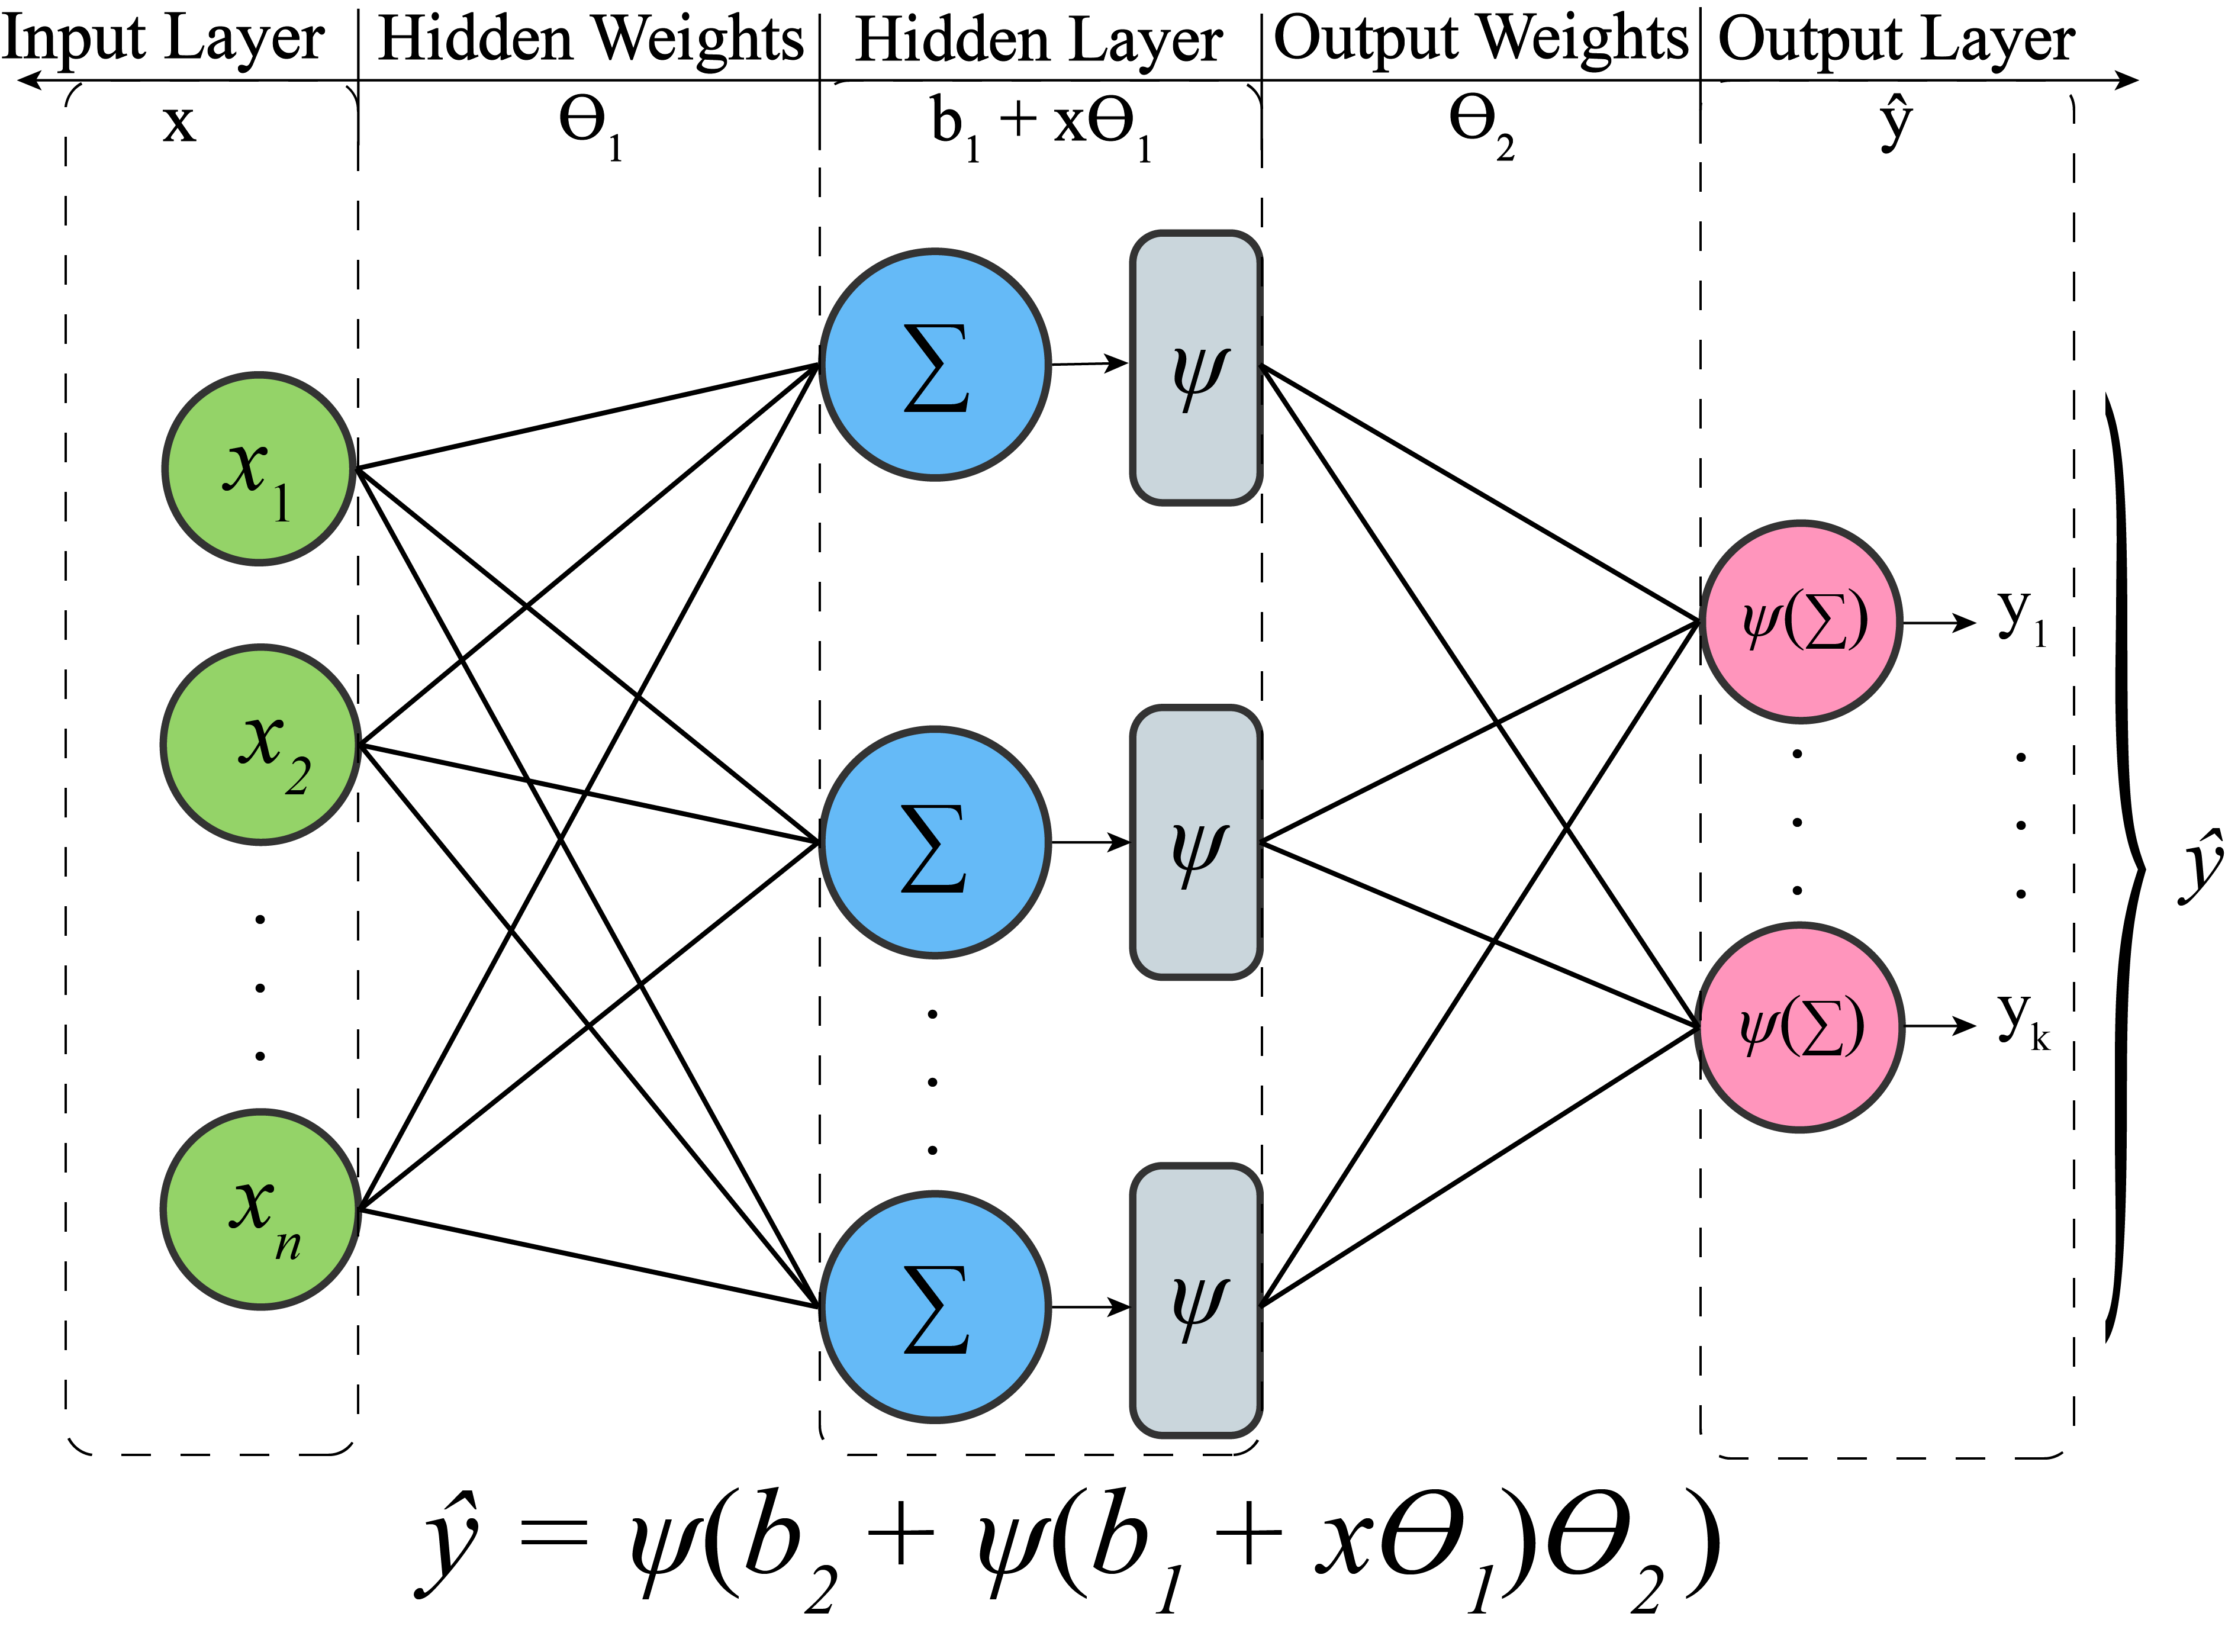
\includegraphics[height = 6cm, width=\textwidth]{img/mlp.png}
        \caption{Feed Forward Multilayer Perceptron}
        \label{fig:mlp}
    \end{subfigure}
    \hfill
    \begin{subfigure}[b]{0.40\textwidth}
        \includegraphics[height = 6cm, width=\textwidth]{img/actfunc.png}
        \caption{Common Activation Functions, $\psi$}
        \label{fig:actfunc}
    \end{subfigure}
    \caption{\ref{fig:mlp}) Structure of a feed forward MLP with three layers. \ref{fig:actfunc}) The output for Logistic, Tanh and ReLU activation functions for input value range [-4,4].}\label{fig:mlp_actfunc}
\end{figure}
% Change the italics brackets to regular 
% Add activation function to hidden layer 
% 
%Define supervised classification and regression before hand

A nonlinear activation function $\psi$ allows the compositional output function $ \hat{y}$ to map inputs non-linearly to outputs. Deeper MLPs will contain many more hidden layers then displayed in Figure \ref{fig:mlp} and a neural network with $n$ layers can be defined recursively as:
\begin{equation}
        \hat{y} = \psi(\theta_{n}(\psi(\theta_{n-1}(\psi(\theta_{n-2}(\ldots \psi(\theta_{1} x + b_{1}) \ldots)) + b_{n-2})) + b_{n-1}) + b_{n}) 
\end{equation}

Where the structure of $\hat{y}$ depends on the desired task (e.g nonlinear regression or classification). For regression problems, $\hat{y}$ is a real value, and for classification problems, $\hat{y}$ is a $k$ dimensional vector of real values. So although it is generally advantageous for hidden units to have nonlinear activation functions, the choice of activation functions for output layers will largely depend on the desired task. For nonlinear regression, a linear activation function is generally adequate. However, in classification problems, it can be useful to view the $k$ dimensional output vector $\hat{y} = (y_1,y_2,..., y_k)$ as providing the probabilities a given input example resides in each respective class. This produces a probability distribution over the $k$ classes, where entries fall between $(0,1)$, and the sum of the vector $\hat{y}$ is one. This behaviour can be accomplished by the softmax function:
\begin{equation}
       softmax(z) =  \frac{e^{z_j}}{\sum_{i=1}^{k}e^{z_i}} \;\;\; \mbox{for} \;\;\; j = 1,\ldots,k
\end{equation}

Where $softmax(z)$ represents the categorical distribution of arbitrary $k$ dimensional vector $z$. Furthermore, with a formally defined arbitrary output function $\hat{y}$, the next step requires the artificial neural network to learn weights and biases in order to produce desired outputs given input data.

\subsubsection{The Cost Function}
Training an artificial neural network relies on determining the network parameters that minimize the error between outputs $\hat{y}$ and true values $y$. This entails producing a model function, that given inputs, can produce the output to the closest degree. In machine learning, the notion of a good model is explicitly defined using some cost function $J(\hat{y},y;\Theta)$, where $\Theta = \{\theta, b\}$ is the set of all network weights and biases. The cost function keeps track of the model's prediction error, and finding better models equates to finding better network parameters that minimizes the cost function. For nonlinear regression, a commonly used measure of cost is simply the mean squared error between the output of the neural network and the true values:
\begin{equation} \label{eq:mse} 
    J(\hat{y},y;\Theta) = \sum_{i=1}^{m}(y_i - \hat{y_i})^{2}
\end{equation}

For classification problems, it is often beneficial to represent categorical true labels $y$ as binary vectors. This is referred to as one hot encoding, where the $i$th position of class $i$ is one, and every other term is zero. For example, in a five class problem, a class of three would be coded as $y = [0,0,1,0,0]$. In this way, the error must be calculated for each potential class $k$ over all examples in the sample set. Accordingly, the most commonly used cost function for classification problems is the cross entropy loss:
\begin{equation} \label{eq:softmax}
    J(\hat{y}, y; \Theta) = - \frac{1}{m}\sum_{i = 1}^{m}\sum_{j = 1}^{k} \lbrack y_{i,j} \log(\hat{y_{i,j}}) + (1 - y_{i,j})\log(1 - \hat{y_{i,j}}) \rbrack
\end{equation}

In the computation of cross-entropy loss, $k$ error terms are generated for every training example. The cross-entropy loss represents the log probability of classes given the model - that is, maximizing the likely hood of a training example belonging to a specific class is equivalent to minimizing the cross entropy loss between $\hat{y}$ and $y$. 

\subsubsection{The Optimization Algorithm}
The cost, $J(\hat{y}, y; \Theta)$, is conveniently a function of the training examples and model parameters $\Theta$. In order to effectively minimize the cost function, it is useful to observe how the cost changes with respect to weights $\theta$. Formally, this is expressed with the partial derivative $\frac{\partial J}{\partial \theta}$. With this expression, we can search for weights in the direction that cost $J$ decreases. This technique, called gradient descent, minimize cost by iteratively updating $\theta$ in the opposite direction of the gradient:
\begin{equation}
    \theta_j = \theta_j - \alpha \frac{\partial}{\partial \theta_j} J(\hat{y},y;\Theta) \;\;\; \mbox{for} \;\;\; j = 1,\ldots,n
\end{equation}

%Other optimization techniques have been developed, but not many of them are shown to generalize performance, andrew ng (gradient descent/adam), an exception is the adam optimizer (reference)  

Where $\alpha$, the learning rate, controls the size of steps made in the direction of the negative gradient. Furthermore, in order to compute the gradients of the cost with respect to model weights, an algorithm called backpropagation is commonly used. The cost function, as one large nested composite function, contains all of the computations in the neural network. With this, the backpropagation algorithm cleverly applies the chain rule of calculus to recursively compute the gradients of each weight, as shown in Figure \ref{fig:backprop}. 

%with respect to the outputs so weights can be updated incrementally using gradient descent. 

\begin{figure}[h!]
    \centering
    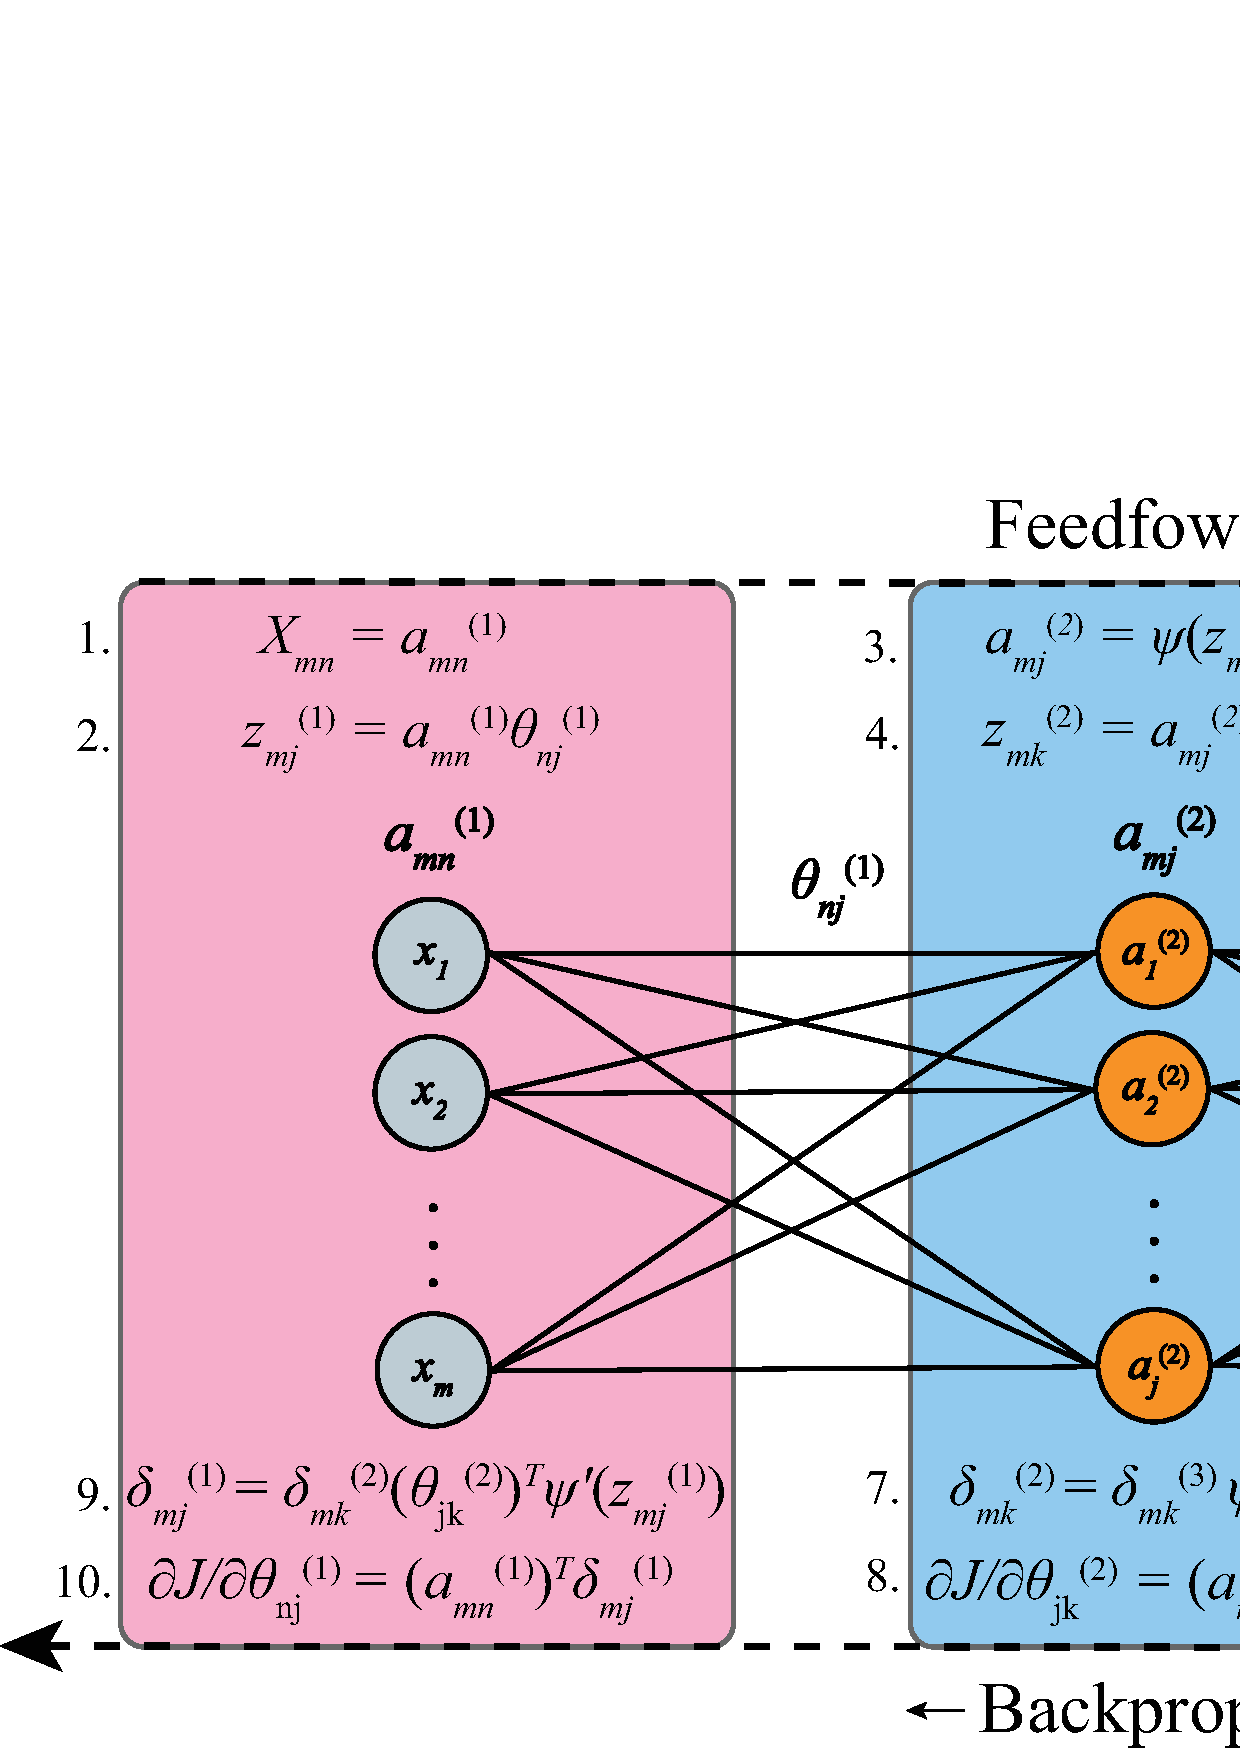
\includegraphics[width=\textwidth]{img/backprop.png}
    \caption{Feedforward and Backpropagation Schematic.}
    \label{fig:backprop}
\end{figure}

%Should I go through an algorithmic overview of this process?
%Or a demonstration with a model neural network?

%Deeper neural networks simply continue to stack these operations 



%In Figure \ref{fig:actfunc}, we see that the tanh and logistic functions have sigmoidal shapes, mapping all inputs between $(-1,1)$ and $(0,1)$, respectively. In the output layer, this kind of behaviour makes them useful for classification problems. Though for nonlinear regression, a linear output activation would be beneficial. Accordingly, the choice of activation functions will largely depend on the desired task, but it is generally desired for the hidden units to have nonlinear activation functions. Deeper MLPs will contain many more hidden layers then displayed in Figure \ref{fig:mlp}, 

%%The cost function, as one large nested composite function, contains all of the computations in the neural network. 

\section{Deep Learning} \label{sec:deeplearning}

\subsection{Deep Neural Networks}

%Explain what deep learning is, why it is used (representation learning)

\subsection{Autoencoders}

%This continues to the stacked denoising variant

Autoencoders represent a family of unsupervised artificial neural networks that learn latent data codings for input data. Here, training examples are utilized without labels, and autoencoders are trained to generate outputs identical to the inputs. The role of an autoencoder is split into two tasks, encoding and decoding. The process of encoding maps the input to lower dimension features, and decoding maps the encoded data back into the original space. The mapping of an input layer produced by function, $g_{\theta}(\cdot)$, can be expressed as:
 
\begin{equation}
z = g_{\theta}(x) = \psi(\theta x + b)
\end{equation}

This latent layer, of potentially reduced dimensionality, can then be decoded back to the original space with function $f_{\theta^{T}}(\cdot)$:

\begin{equation}
x' = f_{\theta^{T}}(z) =  f_{\theta^{T}}(g_{\theta}(x)) = (\theta^{T}z + b)
\end{equation}

Where $x'$ is the reconstructed input data, and $\theta^{T}$ is the transpose of weights used for encoding. Furthermore, to train the model, the reconstructed output is compared to the original input using the mean squared error to calculate reconstruction error:

\begin{equation}
J(x'_{i},x_{i};\Theta) = \frac{1}{2m}{\sum^{m}_{i=1}} ||x_i - x'_i||^2
\end{equation}

Where $\Theta = \{\theta, b_\theta,\theta^{T}, b_{\theta^{T}}\}$ is the set of network parameters used for encoding and decoding operations. 

\subsubsection{Denoising Autoencoders}
Training an autoencoder with partially corrupted data while comparing the reconstruction to the original input is a commonly used technique to increase the robustness of an autoencoder. This modification produces a variant of the basic autoencoder called a denoising autoencoder. By adding corruption to the input data, $\tilde{x}_{i} \sim \mu_{D}(\tilde{x}_{i}|x_{i})$, the autoencoder must learn parameters that can overcome stochastic noise. The operation $\mu_{D}$ defines the form of noise used to corrupt the input data, and the reconstruction error is calculated using cost $J(\tilde{x}'_{i},x_{i};\Theta)$. 

Furthermore, deeper frameworks of denoising autoencoders, called stacked denoising autoencoders (SDAEs), are employed to increase the number of latent abstractions. SDAEs are composed of multiple layers of incrementally stacked denoising autoencoders that are trained one layer at a time. In this way, once the $k$th hidden layer is trained, layer $k+1$ can be trained using the $k$th layer as the input data.

% Add figures for stacked denoising autoencoder
% Add figure for variational autoencoder

%\subsubsection{Variational Autoencoders}

\section{Improving Machine Learning Models}

\subsection{Regularization}
%Talk about overfitting
%Regularization

\subsection{Model Averaging}
%Model Averaging - dropout and maxout model

\section{Information Fusion}

\subsection{Mixture of Experts}

\subsection{Gated Multimodal Units}




    \chapter{Related Work} \label{chap:relatedwork}
    \chapter{Deep Gated Multimodal Units} \label{chap:deepgmu}

In this chapter we propose a novel multimodal fusion approach to integrate information from multiple genomic sources. While most methods have solely relied on data fusion (early fusion) or decision level fusion (late fusion), our approach utilizes a series of cascading gated multimodal units to deeply connect the integration of data fusion and decision fusion.
%by a series of cascading layers

\section{Architecture}

The architecture of a dGMU first contains multiplicative gates designed to construct an intermediate representation of data from multiple modalities. The input modalities along with the intermediate representation are then fed to a decision network that fuses the predictions using an additional gate. These two processes can be subdivided into the function of a representation network and a decision network. In the representation network, the input modalities learn a latent representation of the combined input data. While the decision network makes predictions based on all representations and learns to decide how decisions influence the activation of the output unit. This structure is illustrated in Figure \ref{fig:dgmu}. 

\begin{figure}[h!]
    \centering
    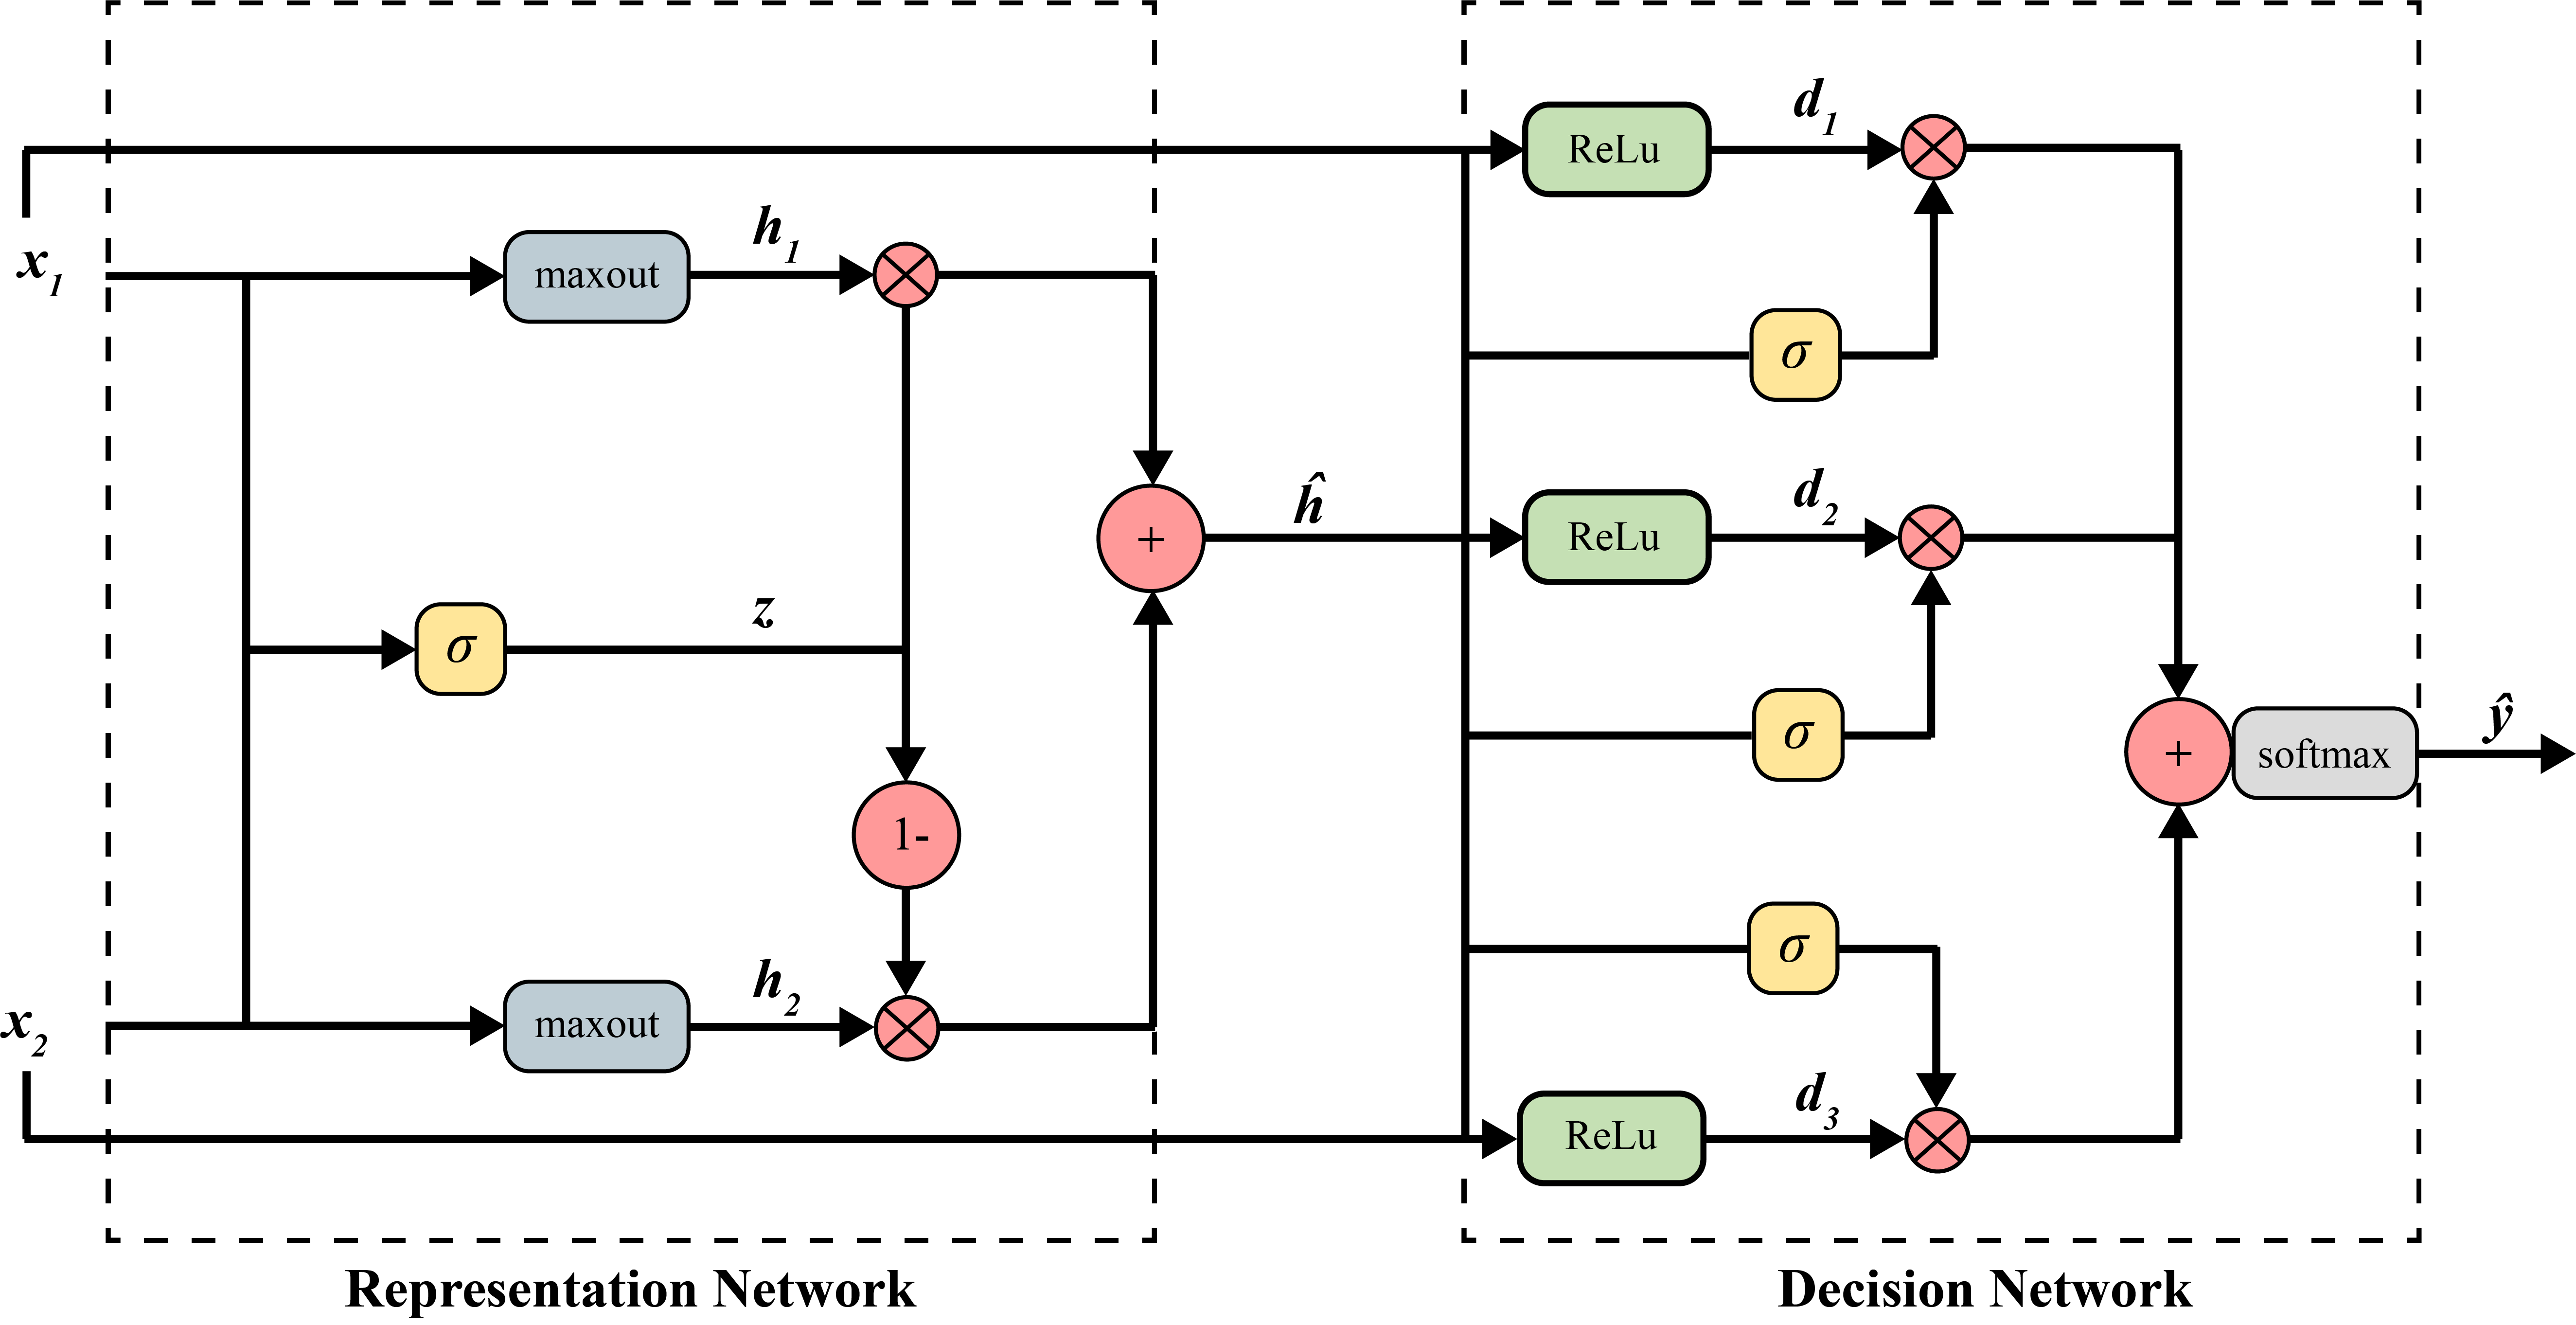
\includegraphics[width=\textwidth]{img/dGMU.png}
    \caption{Deep Gated Multimodal Unit.}
    \label{fig:dgmu}
\end{figure}

\noindent
The connection between the internal representation and decision networks are governed by the following equations:

\noindent
\textbf{Representation Network}
\begin{center}
    $h_1 = maxout(\theta_{h1} \cdot x_1)$\\
    $h_2 = maxout(\theta_{h2} \cdot x_2)$\\
    $z = \sigma(\theta_z \cdot [x_1,x_2])$\\
    $x_3(x_1,x_2;\Theta_R) = z * h_1 + (1-z)*h_2$\\
    %$\Theta_R = \left\{W_{h1},W_{h2},W_{x3}\right\}$\\
\end{center}

\noindent
Where latent space, $x_3(x_1,x_2;\Theta_R)$, depends on inputs $x_1$ and $x_2$, and $\Theta_R = \left\{\theta_{h1},\theta_{h2},\theta_{x3}\right\}$ is the set of network parameters used for encoding the latent space.

\noindent
\textbf{Decision Network}

\begin{center}
    $$
        \hat{y}(x_1,x_2,x_3;\Theta_D) = {\sum^{3}_{i=1}} ReLu(\theta_{di} \cdot x_i)\sigma(\theta_{di} \cdot [x_1,x_2,x_3])
    $$\\   
    %$\Theta_D = \left\{W_{d1},W_{d2},W_{d3},W_{g1},W_{g2},W_{g3}\right\}$\\
\end{center}

\noindent
Where the network output, $\hat{y}(x_1,x_2,x_3;\Theta_D)$, depends on inputs $x_1$, $x_2$, and $x_3$, and $\Theta_D = \left\{\theta_{d1},\theta_{d2},\theta_{d3},\theta_{g1},\theta_{g2},\theta_{g3}\right\}$ is the set of network parameters used across the untied gates in the decision network.

%Internal gating neuron
%representation network
%decision network

\section{Training}

%majahan

The dGMU model parameters were learned with batch stochastic gradient descent with ADAM optimization \cite{kingma2014adam}. The training complexity was reduced by using a supervised pre-training scheme on the decision network \cite{mahajan2018exploring}. This method is used to initialize the parameters of the decision network to ease the training of the larger model, reducing computation time and increasing model robustness \cite{clune2013evolutionary}. The complete network was optimized using supervised fine-tuning with the connected sub-networks. During the training process, overfitting was controlled using dropout and $L_2$ regularization. For classification problems the global loss is computed using the softmax cross entropy loss as seen in Equation \ref{eq:softmax}. With regularization, this results in the following global loss:

\begin{equation}
    Loss = - \frac{1}{m}\sum_{i = 1}^{m}\sum_{j = 1}^{k} \lbrack y_{i,j} \log(\hat{y_{i,j}}) + (1 - y_{i,j})\log(1 - \hat{y_{i,j}}) \rbrack + \frac{\lambda}{2m} \sum_{j = 1}^{p}\sum_{k = 1}^{q}\Theta^{2}_{j,k}
\end{equation}

\section{Implementation}

The dGMU model was implemented with original code in Tensorflow (1.11.0) on an Nvidia Tesla K80 GPU. With a high level of parallization and batch training used during pretraining and finetuning, the model training takes a few minutes, and validation and testing is conducted in a matter of seconds.

The dGMU model benefits from the modularity of gated multimodal units. Accordingly, this architecture can be adapted using varying models for each modality depending on the application. As well, the decision network can be modified to accept inputs from more than two modalities while only resulting in a linear increase in the number of training weights.

Furthermore, this model generates a latent space in between the representation network and the decision network. This offers an interesting avenue into investigating the biological significance of the fused latent representation. 
    \chapter{Materials and Methods} \label{chap:experiments}

\section{Genomic Data Preprocessing}

In this report, all genomic data was acquired from the National Cancer Institutes (NCI) genomic data portal \cite{grossman2016toward}. Healthy and tumorous cell mass RNA expresssion, microRNA expression, copy number variation, and simple nucleotide variation data was acquired for nine different forms of cancer and solid tissue normal (STN) samples. The nine cancer types included were head and neck squamous cell carcinoma (HNSC), kidney renal clear cell carcinoma (KIRC), kidney renal papillary (KIRP), liver hepatocellular carcinoma (LIHC), lung adenocarcinoma (LUAD), lung squamous cell carcinoma (LUSC), prostate adenocarcinoma (PRAD), thyroid carcinoma (THCA). The following subsections detail the preprocessing steps required to transform and extract features from the raw genomic data.

\subsection{Copy Number Variation}

\subsubsection{Preprocessing}

The copy number variation (CNV) data was derived from somatic and germline genotyping array (Affymetric Genome-Wide Human SNP Array 6.0). The raw CNV data is given as segmented genomic regions that have the same DNA copy number. This form provides the number of bound probes and the binary logarithm of the mean intensity (segmented mean) for each segmented genomic region as shown in Table \ref{table:rawcnv}.

\begin{table}[ht]
\caption{Raw CNV Data from Genome Wide SNP Segmentation} % title of Table
\centering % used for centering table
\resizebox{\textwidth}{!}{% % force table to text width
\begin{tabular}{l l l l l l} % centered columns (4 columns)
\hline %inserts single horizontal lines
GDC Aliquot $^a$ & Chr & Start & End & Probes & Segment Mean\\ %[0.5ex] % inserts table
%heading
\hline % inserts single horizontal line
% inserting body of the table
00e5b006-6afc-4ea4-90e3-f29741560020 & 1 & 62920 & 814954 & 31 & 0.4742\\
00e5b006-6afc-4ea4-90e3-f29741560020 & 1 & 817186 & 3303537 & 710 & -0.0539\\
00e5b006-6afc-4ea4-90e3-f29741560020 & 1 & 3303596 & 16477281 & 7873 & 0.0117\\
00e5b006-6afc-4ea4-90e3-f29741560020 & 1 & 16477846 & 16935737 & 127 & 0.3408\\
00e5b006-6afc-4ea4-90e3-f29741560020 & 1 & 16935752 & 30261189 & 7664 & 0.0229\\
% [1ex] adds vertical space
\hline %inserts single line
\end{tabular}}
\raggedright
\footnotesize{$^a$ Aliquot cooresponds to KIRC primary tumour UUID 0063a6fa-9ebd-4b71-83c0-aeb17b97eb6.}

\label{table:rawcnv}
\end{table}


\noindent
In order to extract features that can be shared between all ten cell mass types, the chromosomal regions were mapped to genes. Using the BioMart community portal we acquired the start and end positions of every gene in the human genome assembly GRCh38 (hg38) \cite{smedley2015biomart}. The human genes were then mapped to the CNV regions for each sample type. An example of the resulting process is shown in Table \ref{table:mapgene}.

\begin{table}[ht]
\caption{Significant CNV Abberations Mapped to Gene Ensembl ID in KIRC} % title of Table
\centering % used for centering table
\resizebox{\textwidth}{!}{%
\begin{tabular}{l l l l l l} % centered columns (4 columns)
\hline %inserts single horizontal lines
Ensembl ID & Chr & Abberration & Segment Mean & CNV Region & Gene Region\\ %[0.5ex] % inserts table
%heading
\hline % inserts single horizontal line
% inserting body of the table
ENSG00000237763 & 1 & DEL & -1.361 & 103620877-103717410 & 103655290-103664554\\
ENSG00000244057 & 1 & DEL & -1.9195 & 152583230-152613762 & 152600662-152601086\\
ENSG00000198502 & 6 & DUP & 1.9859 & 32488906-32533522 & 32517343-32530287 \\ 
ENSG00000264892  & 17 & DEL & -2.8409 & 16806233-16815664 & 16812447-16812651\\
ENSG00000279442 & 22 & DUP & 2.0311 & 15294547-15315221 & 15298378-15304556\\ 
% [1ex] adds vertical space
\hline %inserts single line
\end{tabular}}
\label{table:mapgene}
\end{table}

% GeneSymbol
% N/A
% AMY1A
% LCE3C
% HLA-DRB5
% NOS2P4
%Extra, just in case the Ensembl IDs dont fit
%TRGV4: ENSG00000211698 & 7 & DEL & -2.0425 & 38351764-38356875 & 38353715-38354517

\subsubsection{Dataset}

For the $i$-th cell mass, a set of $g_i$ genes were mapped to aberrant regions within the genome. The set of common genes between all cell mass types were defined as:

\begin{equation}
    g = g_i \cap g_{i+1} \;\;\; \mbox{for} \;\;\; i = 1,\ldots,n
\end{equation}

\noindent
Where $n$ is the number of cell mass samples. As a result, the CNV data contained the segmented mean of 11479 genes for each cell mass sample, resulting in a processed data matrix $C \in {\rm I\!R}^{11479 \; x \; n}$.

\subsection{Transcriptome Expression}

\subsubsection{Preprocessing}

This study utilized RNA sequence (RNA-seq), and microRNA sequence (miRNA-seq) transcriptome expression profiling. MiRNA-seq is a form of transcriptome profiling that provides miRNA molecule quantification. The miRNA-seq data used in this study was derived using the BCGSC miRNA profiling pipeline \cite{chu2015large}. Furthermore, RNA-seq is a form of transcriptome profiling that provides gene expression quantification. The RNA-seq data used in this study was derived from HTSeq-Counts framework \cite{anders2015htseq}.

All expression profiles were organized in relation to cancer subclass, individual case ID, and sequence ID. An example of this is shown in Figure \ref{fig:expmirna}.

\begin{figure}[h!]
    \centering
    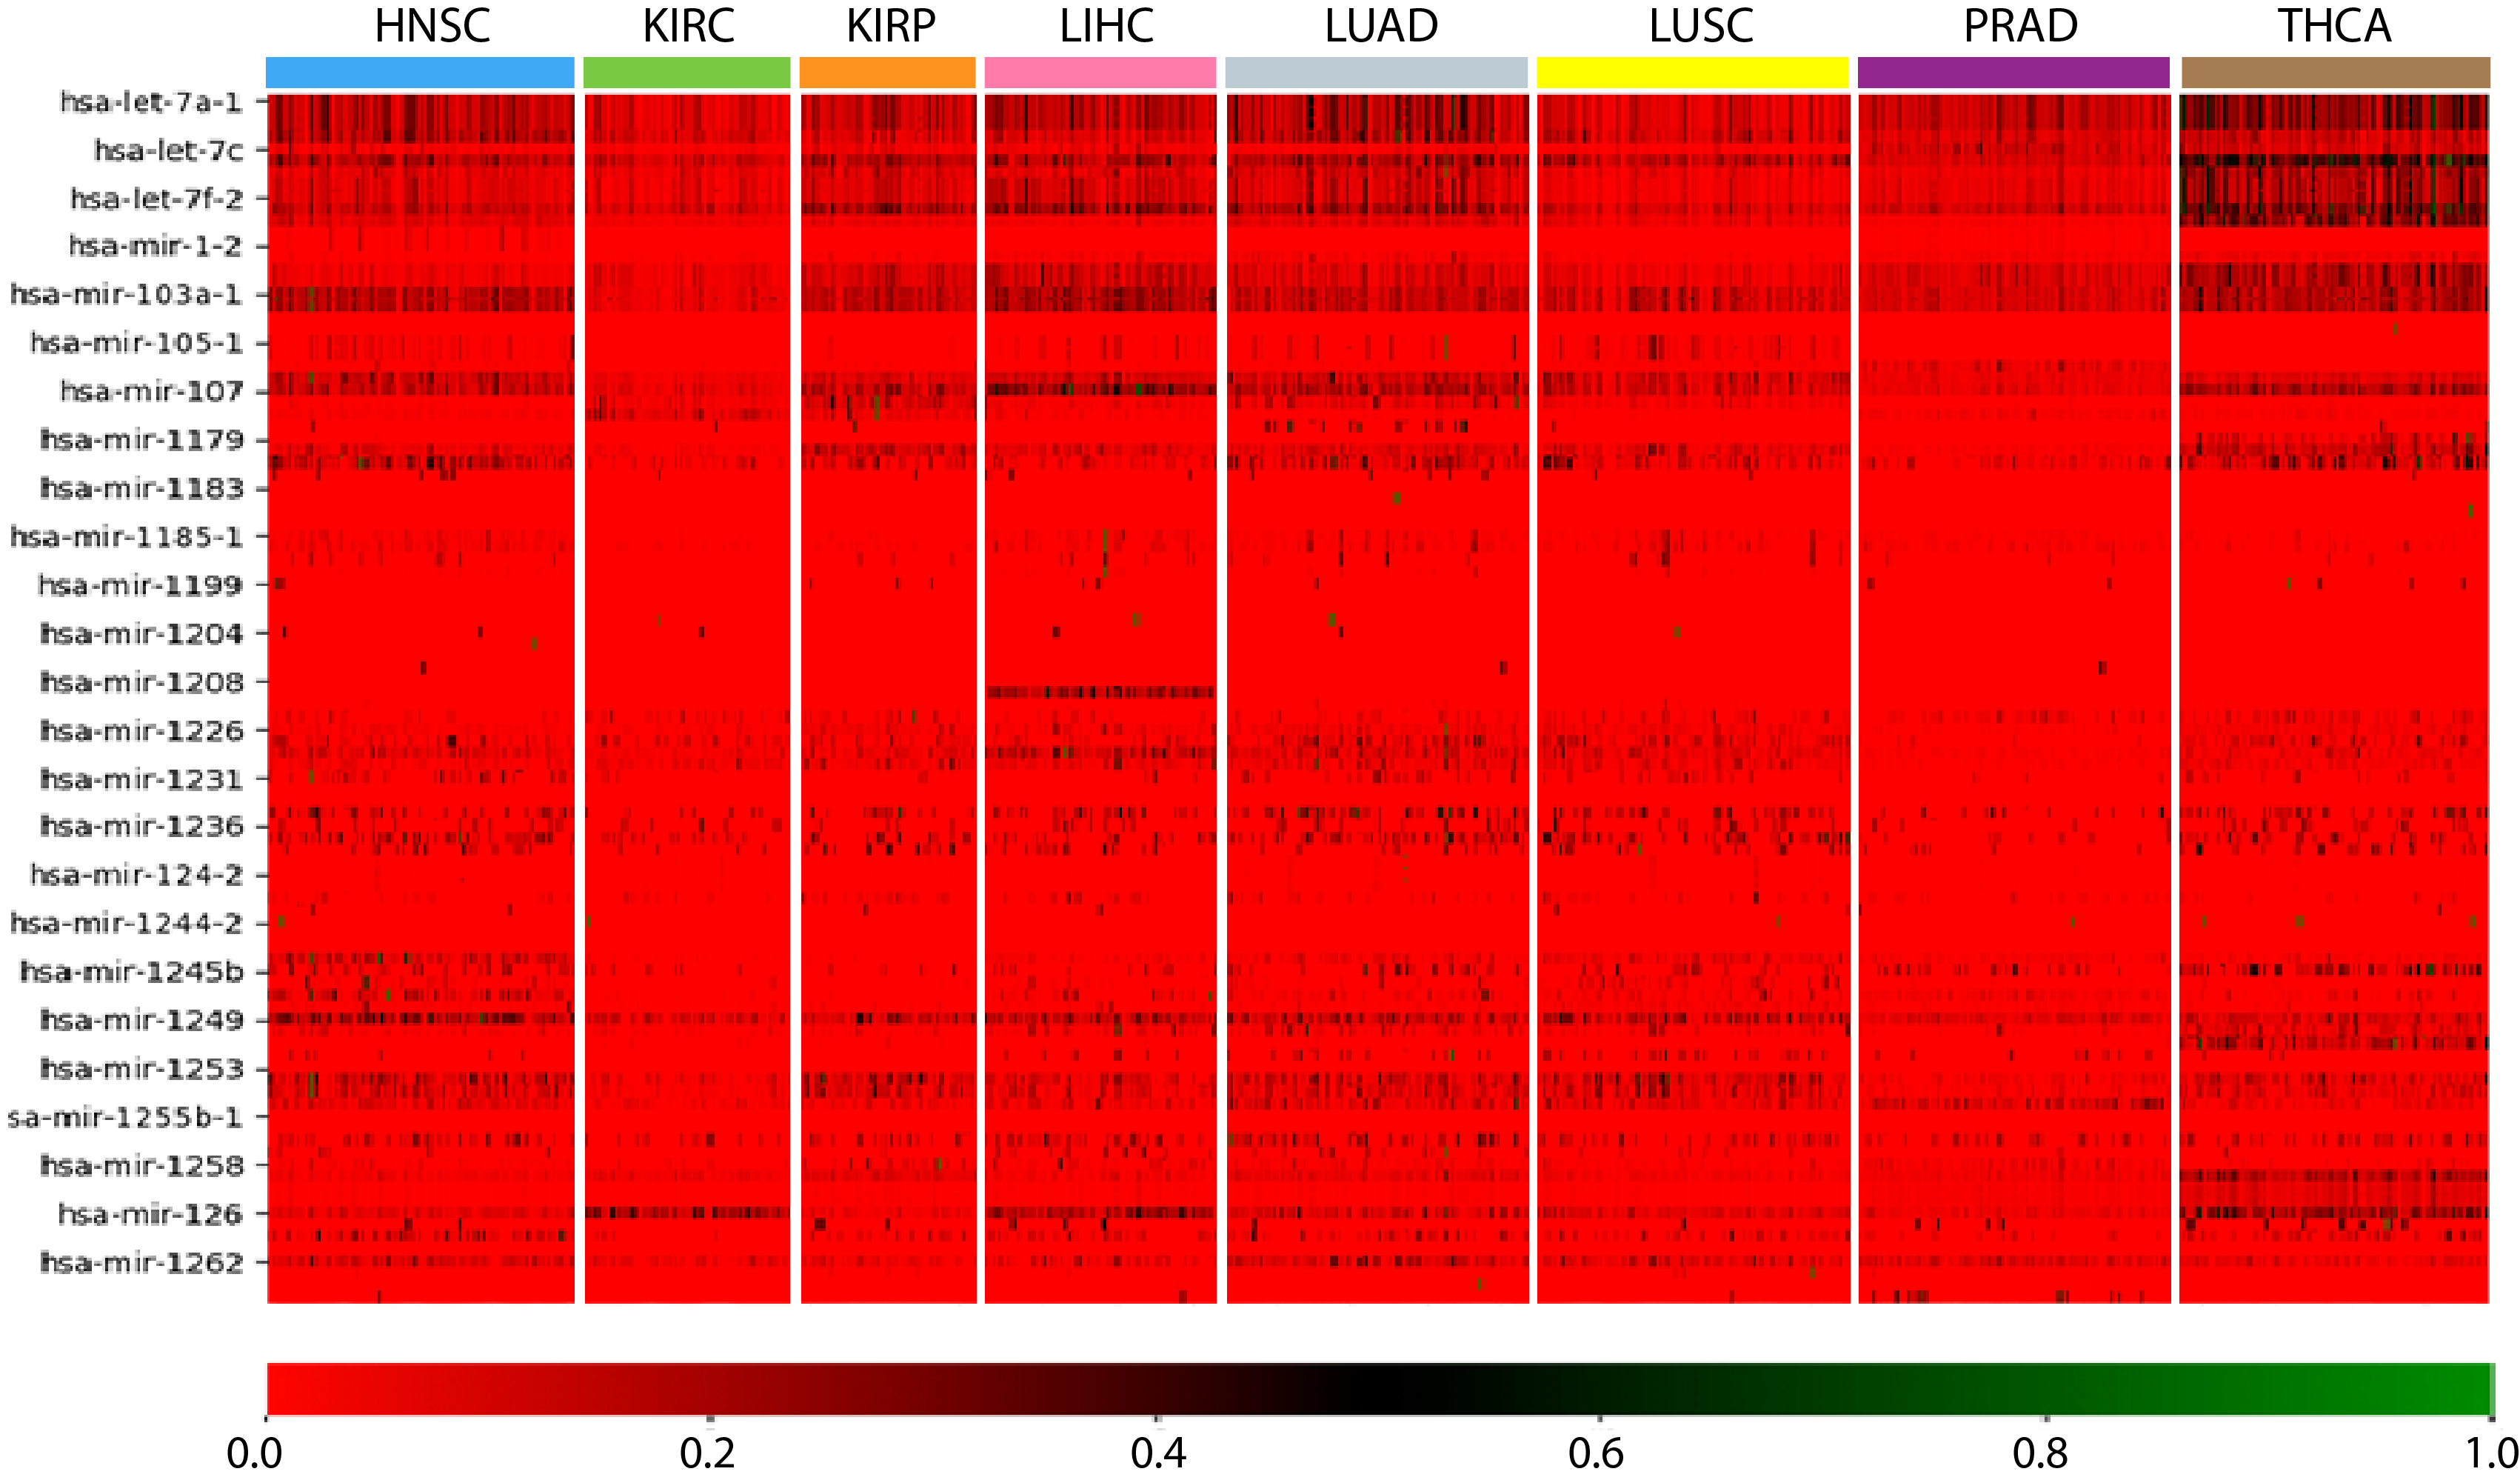
\includegraphics[width=\textwidth]{img/expmirna.png}
    \noindent
    \caption{Normalized miRNA expression profiles.}
    \label{fig:expmirna}
\end{figure}

\subsubsection{Dataset}

The expression profiles of the transcriptome expression data had the input feature dimensionality of all assayed genes and miRNA molecules. The miRNA-seq expression data contained the normalized expression counts of 1881 miRNA molecules, while the RNA-seq expression data contained the normalized expression counts of 60484 genes. As a result, the processed miRNA-seq data produced data matrix $M \in {\rm I\!R}^{1881 \; x \; n}$, and the processed RNA-seq data produced data matrix $R \in {\rm I\!R}^{60484 \; x \; n}$.

\subsection{Simple Nucleotide Variation}

\subsubsection{Preprocessing}

The simple nucleotide variation (SNV) data was obtained in the form of masked somatic mutations, derived from a MuTect2 Variant Aggregation and Masking workflow \cite{cibulskis2013sensitive}. 

\begin{figure}[h!]
    \centering
    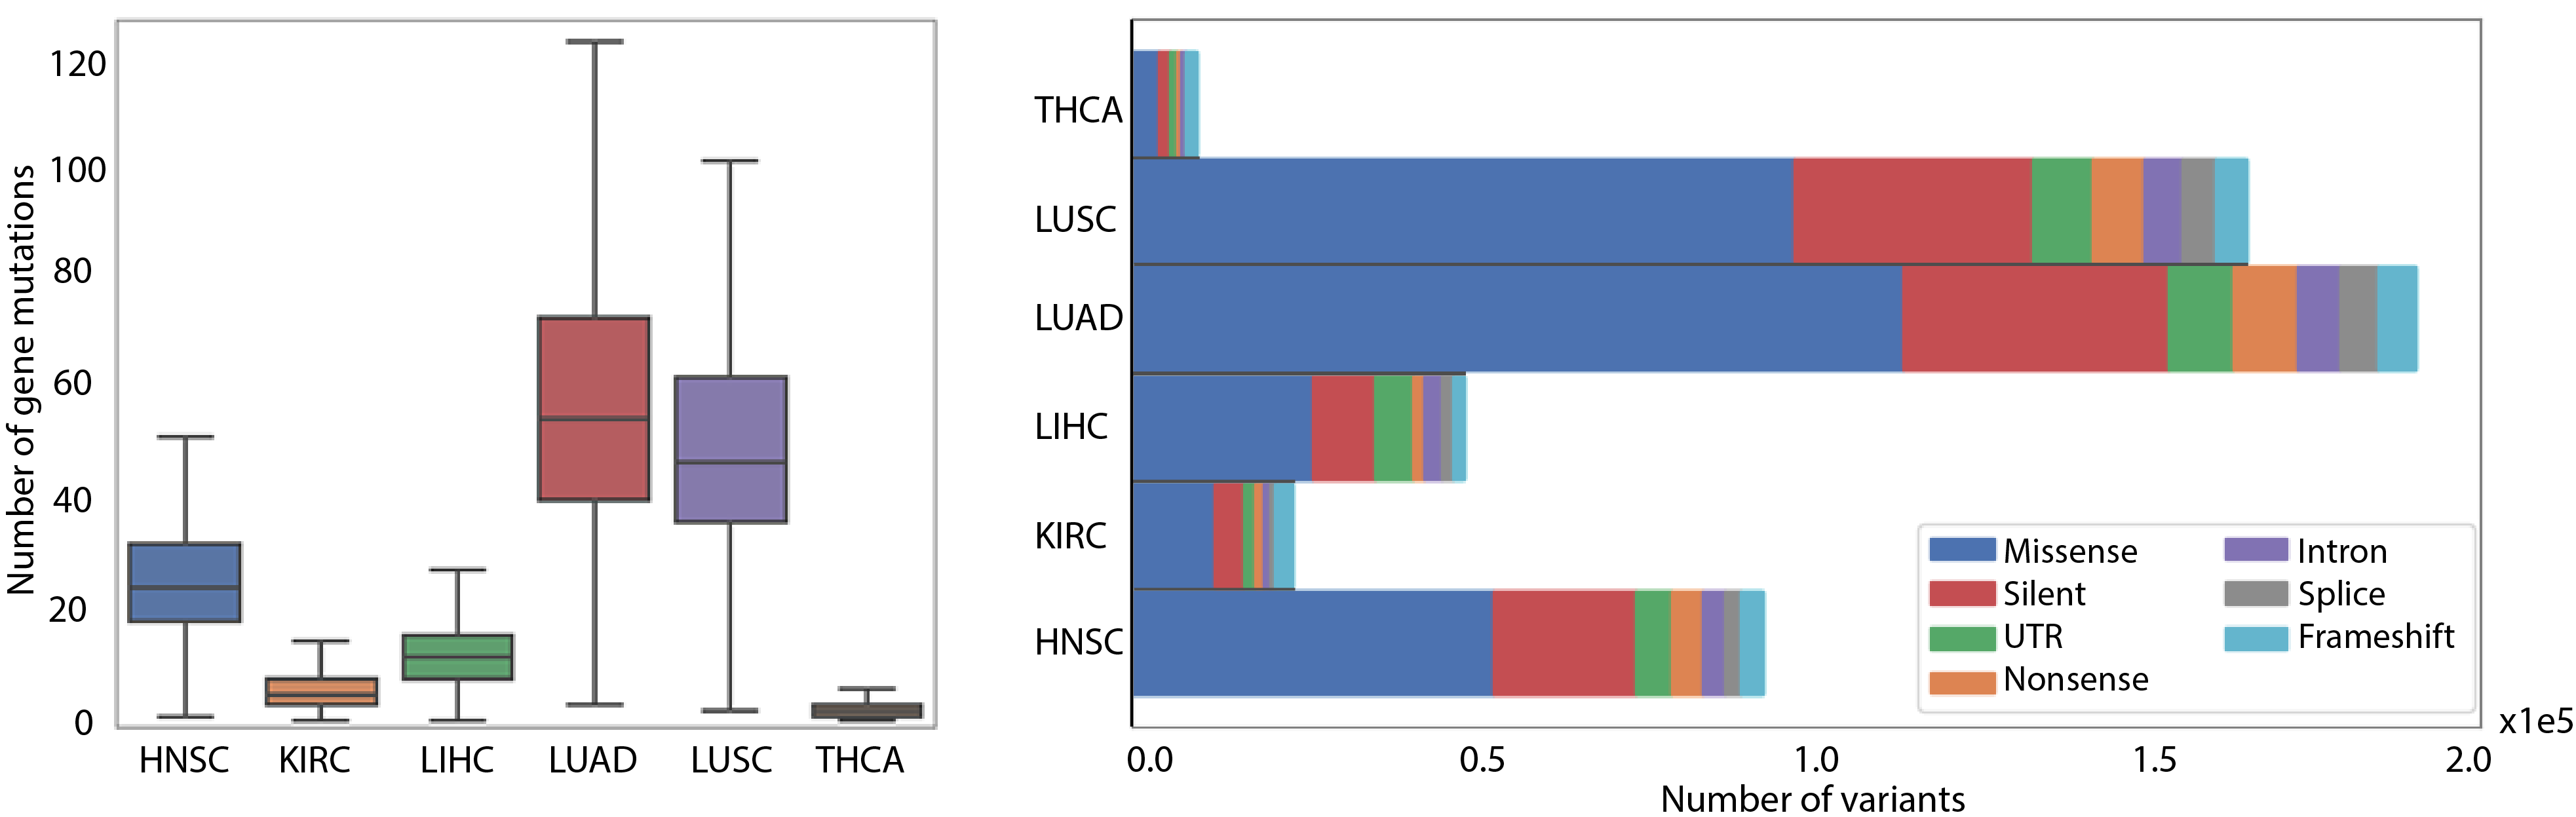
\includegraphics[width=\textwidth]{img/snvstats.png}
    \noindent
    \begin{minipage}[t]{.39\textwidth}
    \raggedright
        a) Accumulated gene mutations
    \end{minipage}% 
    \hspace{1cm}
    \begin{minipage}[t]{.5\textwidth}
        b) Variant classification distribution
    \end{minipage}
    \centering
    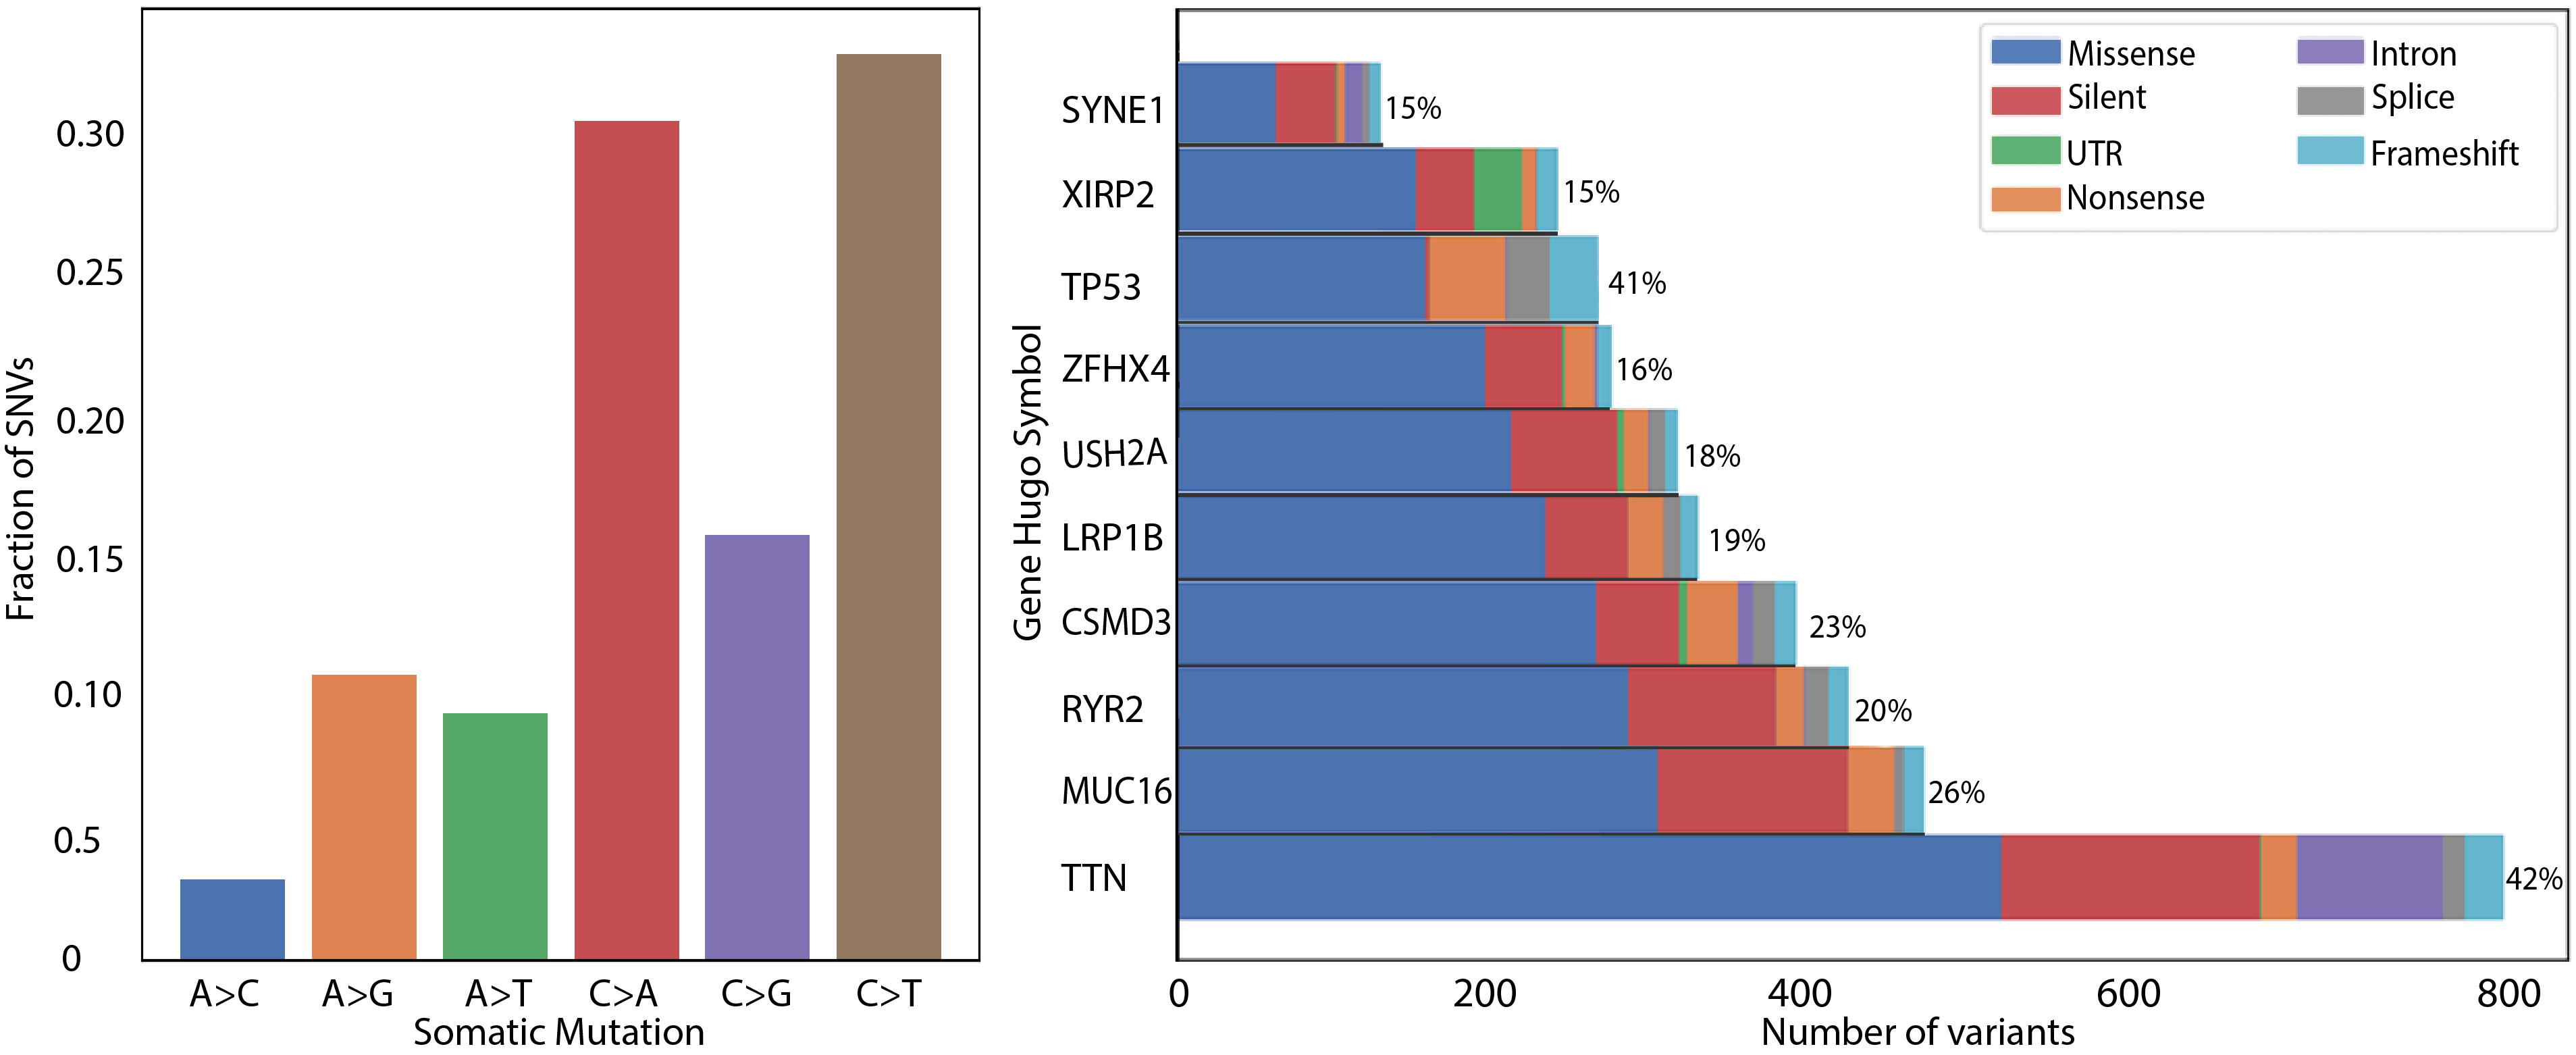
\includegraphics[width=\textwidth]{img/snvstats2.png}
    \noindent
    \begin{minipage}[t]{.39\textwidth}
    \raggedright
        c) Fraction of somatic muations
    \end{minipage}% 
    \hspace{1cm}
    \begin{minipage}[t]{.5\textwidth}
        d) Variant distribution of top 10 mutated genes
    \end{minipage}
    \caption{a) Box plot of accumulated gene mutations for each cancer type. b) Stacked bar plot showing the distribution of variant classification for each cancer type. c) Bar plot showing the fraction of all somatic mutations. d) Stacked bar plot detailing the distribution of the top 10 mutated genes.}
    \label{fig:snvstats}
\end{figure}
%Number of gene mutations per cancer class.



%number of mutations per cancer class vs fraction mutated

In this study, the analysis of the raw SNV data was based on the variant occurrence frequency of thke genetic data. Variation occurence was mapped to every listed gene for all available cell samples. This was performed by mapping mutated genes to cell sample IDs in the raw SNV data, and accumulating the number of mutations for each respective cell sample.

\subsubsection{Dataset}

After preprocessing the SNV data, the variant occurrence frequency was obtained for 20516 human genes for each cell mass sample. The variant occurrence frequency was recorded in matrix $S \in \{\mathbb{Z}_{\geq 0}\}^{20516 \; x \; m}$, where the 20516 rows coorespond to genes, and the m columns correspond to the m cell samples per gene. Accordingly, a field within matrix $S$ indicates the number of mutations observed for a cell on a given gene. 

\section{Dimensionality Reduction}

In the following, we describe the various forms of dimensionality reduction used to deal with the high dimensionality of the genomic data and the selection of relevant features. 

\subsection{Stacked Denoising Autoencoder}

A SDAE was used to acquire compressed feature vectors from all genomic data sources. A two layer SDAE with dimensions 1000, and 500 was trained using a designated training set. Optimal model parameters were selected based on model performance during 10-fold cross validation. Post training, a layer with reduced dimensionality and a low cross validation error was selected. The defined objective here was to acquire a reduced mapping that encodes the original data with minimal loss of meaningful patterns.

\subsection{Deeply Connected Genes}
The weights of the trained SDAE were used to extract the raw features most strongly connected to the reduced subspace for CNV, RNA-seq and miRNA-seq data sources. These features were extracted from the SDAE by computing the product of the weight matrix for each layer \cite{danaee2017deep}. 
The product of the weights for each layer in the trained and optimally parametized SDAEs were observed to be highly normally distributed as shown in Figure \ref{fig:zscoreHist}. 

\begin{figure}
     \centering
     \begin{subfigure}[b]{0.3\textwidth}
         \centering
         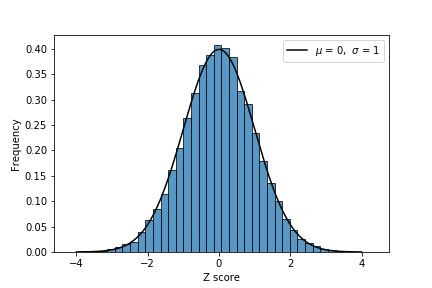
\includegraphics[width=\textwidth]{img/zscoreCNV.png}
         \caption{}
     \end{subfigure}
     \hfill
     \begin{subfigure}[b]{0.3\textwidth}
         \centering
         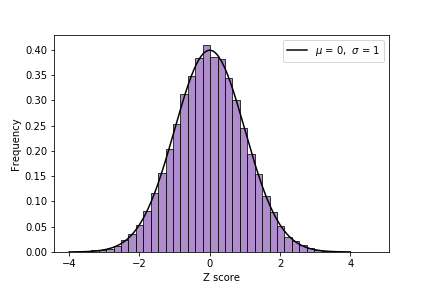
\includegraphics[width=\textwidth]{img/zscoreRNA.png}
         \caption{}
     \end{subfigure}
     \hfill
     \begin{subfigure}[b]{0.3\textwidth}
         \centering
         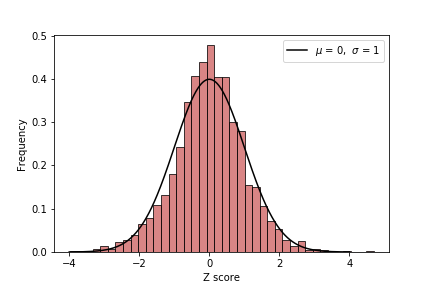
\includegraphics[width=\textwidth]{img/zscoreMIRNA.png}
         \caption{}
     \end{subfigure}
        \caption{Histogram of z-scores from dot product of SDAE weight matrices for a) CNV b) RNA-seq and c) miRNA-seq.}
        \label{fig:zscoreHist}
\end{figure}

The most statistically significant features were identified by fitting the weight matrices to a normal distribution, and computing a p value to select features that match the preselected experimental dimensions.

\subsection{Differential Expression}

For the transcriptome expression data, deferentially expressed genes were identified, and utilized as features. The $log_{2}$(fold change) was computed between the median tumour cell mass expression and healthy cell mass expression. The most statistically significant features were identified by fitting the differential expression to a Guassian distribution and computinbg a two-tailed p-value. Features that match the preselected experimental dimensions were acquired by selected the top most significant deferentially expressed genes using the two-tailed p-values. 

\begin{figure}
     \centering
     \begin{subfigure}[b]{0.49\textwidth}
         \centering
         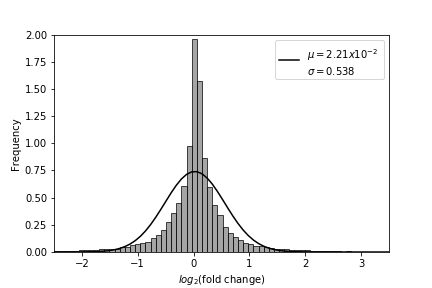
\includegraphics[width=\textwidth]{img/rnaDE.png}
         \caption{}
     \end{subfigure}
     \hfill
     \begin{subfigure}[b]{0.49\textwidth}
         \centering
         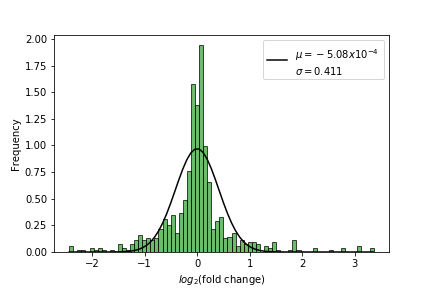
\includegraphics[width=\textwidth]{img/mirnaDE.png}
         \caption{}
     \end{subfigure}
        \caption{Differential expression $log_2$(fold change) and Gaussian fit for a) RNA-seq and b) miRNA-seq.}
        \label{fig:deHist}
\end{figure}

    
\backmatter{}
    \printbibliography



\end{document}

%TODO:
%Add official title page
%Explain backprop figure
%Explain what the percentage in the variant distribution figure is for
